\section{Scale modes}

So far we have seen the major and minor scales. Both the diatonic and pentatonic versions. And all starting from the 6th string. This will allow you to improvise a nice melody over a song.

But, did you realize that the notes in the (diatonic) C major scale (\autoref{tab:guitar_c_major_scale}) and the A minor scale (\autoref{tab:guitar_a_minor_scale}) are the same? That is because the \textbf{relative minor} of a major scale is the 6th index of the scale. In \autoref{tab:guitar_mode_intervals} you can see how to get the minor scale from the major scale.

So does that mean that you can improvise with the A minor scale over a song in C major. YES!. After all, they are the same notes.

Does that mean that C major and A minor are identical. Kinda, but not really. Purely looking at the notes, yes. But when you look at the \textbf{tonal center} (the main note in a melody, or the note that the melody/chord progressions resolves to) than they feel different.

\begin{table}[h]
	\centering
	\begin{tabular}{*{30}{c}}
		Ionian (major) & & \multicolumn{2}{P{4mm}}{\large{W}} & \multicolumn{2}{P{4mm}}{\large{W}} & \multicolumn{2}{P{4mm}}{\large{H}} & \multicolumn{2}{P{4mm}}{\large{W}} & \multicolumn{2}{P{4mm}}{\large{W}} & \multicolumn{2}{P{4mm}}{\large{W}} & \multicolumn{2}{P{4mm}}{\large{H}} & \\
		& \multicolumn{2}{P{4mm}}{\RomanNumeralCaps{1}} & \multicolumn{2}{P{4mm}}{\RomanNumeral{2}} & \multicolumn{2}{P{4mm}}{\RomanNumeral{3}} & \multicolumn{2}{P{4mm}}{\RomanNumeralCaps{4}} & \multicolumn{2}{P{4mm}}{\RomanNumeralCaps{5}} & \multicolumn{2}{P{4mm}}{\RomanNumeral{6}} & \multicolumn{2}{P{4mm}}{\RomanNumeral{7}\textsuperscript{o}} & \\
		\hline \\
		Dorian & \multicolumn{3}{P{4mm}}{} & \multicolumn{2}{P{4mm}}{\large{W}} & \multicolumn{2}{P{4mm}}{\large{H}} & \multicolumn{2}{P{4mm}}{\large{W}} & \multicolumn{2}{P{4mm}}{\large{W}} & \multicolumn{2}{P{4mm}}{\large{W}} & \multicolumn{2}{P{4mm}}{\large{H}} & \multicolumn{2}{P{4mm}}{\large{W}} & \\
		& \multicolumn{2}{P{4mm}}{} & \multicolumn{2}{P{4mm}}{\RomanNumeral{1}} & \multicolumn{2}{P{4mm}}{\RomanNumeral{2}} & \multicolumn{2}{P{4mm}}{\RomanNumeralCaps{3}} & \multicolumn{2}{P{4mm}}{\RomanNumeralCaps{4}} & \multicolumn{2}{P{4mm}}{\RomanNumeral{5}} & \multicolumn{2}{P{4mm}}{\RomanNumeral{6}\textsuperscript{o}} & \multicolumn{2}{P{4mm}}{\RomanNumeralCaps{7}} & \\
		\hline \\
		Phrygian & \multicolumn{5}{P{4mm}}{} & \multicolumn{2}{P{4mm}}{\large{H}} & \multicolumn{2}{P{4mm}}{\large{W}} & \multicolumn{2}{P{4mm}}{\large{W}} & \multicolumn{2}{P{4mm}}{\large{W}} & \multicolumn{2}{P{4mm}}{\large{H}} & \multicolumn{2}{P{4mm}}{\large{W}} & \multicolumn{2}{P{4mm}}{\large{W}} & \\
		& \multicolumn{4}{P{4mm}}{} & \multicolumn{2}{P{4mm}}{\RomanNumeral{1}} & \multicolumn{2}{P{4mm}}{\RomanNumeralCaps{2}} & \multicolumn{2}{P{4mm}}{\RomanNumeralCaps{3}} & \multicolumn{2}{P{4mm}}{\RomanNumeral{4}} & \multicolumn{2}{P{4mm}}{\RomanNumeral{5}\textsuperscript{o}} & \multicolumn{2}{P{4mm}}{\RomanNumeralCaps{6}} & \multicolumn{2}{P{4mm}}{\RomanNumeral{7}} & \\
		\hline \\
		Lydian & \multicolumn{7}{P{4mm}}{} & \multicolumn{2}{P{4mm}}{\large{W}} & \multicolumn{2}{P{4mm}}{\large{W}} & \multicolumn{2}{P{4mm}}{\large{W}} & \multicolumn{2}{P{4mm}}{\large{H}} & \multicolumn{2}{P{4mm}}{\large{W}} & \multicolumn{2}{P{4mm}}{\large{W}} & \multicolumn{2}{P{4mm}}{\large{H}} & \\
		& \multicolumn{6}{P{4mm}}{} & \multicolumn{2}{P{4mm}}{\RomanNumeralCaps{1}} & \multicolumn{2}{P{4mm}}{\RomanNumeralCaps{2}} & \multicolumn{2}{P{4mm}}{\RomanNumeral{3}} & \multicolumn{2}{P{4mm}}{\RomanNumeral{4}\textsuperscript{o}} & \multicolumn{2}{P{4mm}}{\RomanNumeralCaps{5}} & \multicolumn{2}{P{4mm}}{\RomanNumeral{6}} & \multicolumn{2}{P{4mm}}{\RomanNumeral{7}} & \\
		\hline \\
		Mixolydian & \multicolumn{9}{P{4mm}}{} & \multicolumn{2}{P{4mm}}{\large{W}} & \multicolumn{2}{P{4mm}}{\large{W}} & \multicolumn{2}{P{4mm}}{\large{H}} & \multicolumn{2}{P{4mm}}{\large{W}} & \multicolumn{2}{P{4mm}}{\large{W}} & \multicolumn{2}{P{4mm}}{\large{H}} & \multicolumn{2}{P{4mm}}{\large{W}} & \\
		& \multicolumn{8}{P{4mm}}{} & \multicolumn{2}{P{4mm}}{\RomanNumeralCaps{1}} & \multicolumn{2}{P{4mm}}{\RomanNumeral{2}} & \multicolumn{2}{P{4mm}}{\RomanNumeral{3}\textsuperscript{o}} & \multicolumn{2}{P{4mm}}{\RomanNumeralCaps{4}} & \multicolumn{2}{P{4mm}}{\RomanNumeral{5}} & \multicolumn{2}{P{4mm}}{\RomanNumeral{6}} & \multicolumn{2}{P{4mm}}{\RomanNumeralCaps{7}} & \\
		\hline \\
		\textnormal{A}eolian (natural minor) & \multicolumn{11}{P{4mm}}{} & \multicolumn{2}{P{4mm}}{\large{W}} & \multicolumn{2}{P{4mm}}{\large{H}} & \multicolumn{2}{P{4mm}}{\large{W}} & \multicolumn{2}{P{4mm}}{\large{W}} & \multicolumn{2}{P{4mm}}{\large{H}} & \multicolumn{2}{P{4mm}}{\large{W}} & \multicolumn{2}{P{4mm}}{\large{W}} & \\
		& \multicolumn{10}{P{4mm}}{} & \multicolumn{2}{P{4mm}}{\RomanNumeral{1}} & \multicolumn{2}{P{4mm}}{\RomanNumeral{2}\textsuperscript{o}} & \multicolumn{2}{P{4mm}}{\RomanNumeralCaps{3}} & \multicolumn{2}{P{4mm}}{\RomanNumeral{4}} & \multicolumn{2}{P{4mm}}{\RomanNumeral{5}} & \multicolumn{2}{P{4mm}}{\RomanNumeralCaps{6}} & \multicolumn{2}{P{4mm}}{\RomanNumeralCaps{7}} & \\
		\hline \\
		Locrian & \multicolumn{13}{P{4mm}}{} & \multicolumn{2}{P{4mm}}{\large{H}} & \multicolumn{2}{P{4mm}}{\large{W}} & \multicolumn{2}{P{4mm}}{\large{W}} & \multicolumn{2}{P{4mm}}{\large{H}} & \multicolumn{2}{P{4mm}}{\large{W}} & \multicolumn{2}{P{4mm}}{\large{W}} & \multicolumn{2}{P{4mm}}{\large{W}} & \\
		& \multicolumn{12}{P{4mm}}{} & \multicolumn{2}{P{4mm}}{\RomanNumeral{1}\textsuperscript{o}} & \multicolumn{2}{P{4mm}}{\RomanNumeralCaps{2}} & \multicolumn{2}{P{4mm}}{\RomanNumeral{3}} & \multicolumn{2}{P{4mm}}{\RomanNumeral{4}} & \multicolumn{2}{P{4mm}}{\RomanNumeralCaps{5}} & \multicolumn{2}{P{4mm}}{\RomanNumeral{6}} & \multicolumn{2}{P{4mm}}{\RomanNumeral{7}} & \\
	\end{tabular}
	\caption{Mode intervals}
	\label{tab:guitar_mode_intervals}
\end{table}

A mnemonic for the mode name order: \textbf{I} \textbf{D}on't \textbf{P}articularly \textbf{L}ike \textbf{M}odes \textbf{A} \textbf{Lo}t.

\autoref{fig:guitar_diatonic_modes_on_guitar} shows the different mode shapes. In this case the modes of F$\sharp$ are shown. But remember that these can be shifted up or down to be in a different key.

The gray frets with number on the 6th string show the F$\sharp$ major scale on the 6th string. This is used to connect the starting position of the different modes with the major scale indexes. Because we are looking from the major scale's perspective, the numbers in the frets of a shape also correspond to the indexes in the major scale.

Just as before, the different colors indicate different octaves in the shape. Meaning that each shape covers 2 and a bit octaves.

\newpage

\begin{figure}[h]
	\centering
	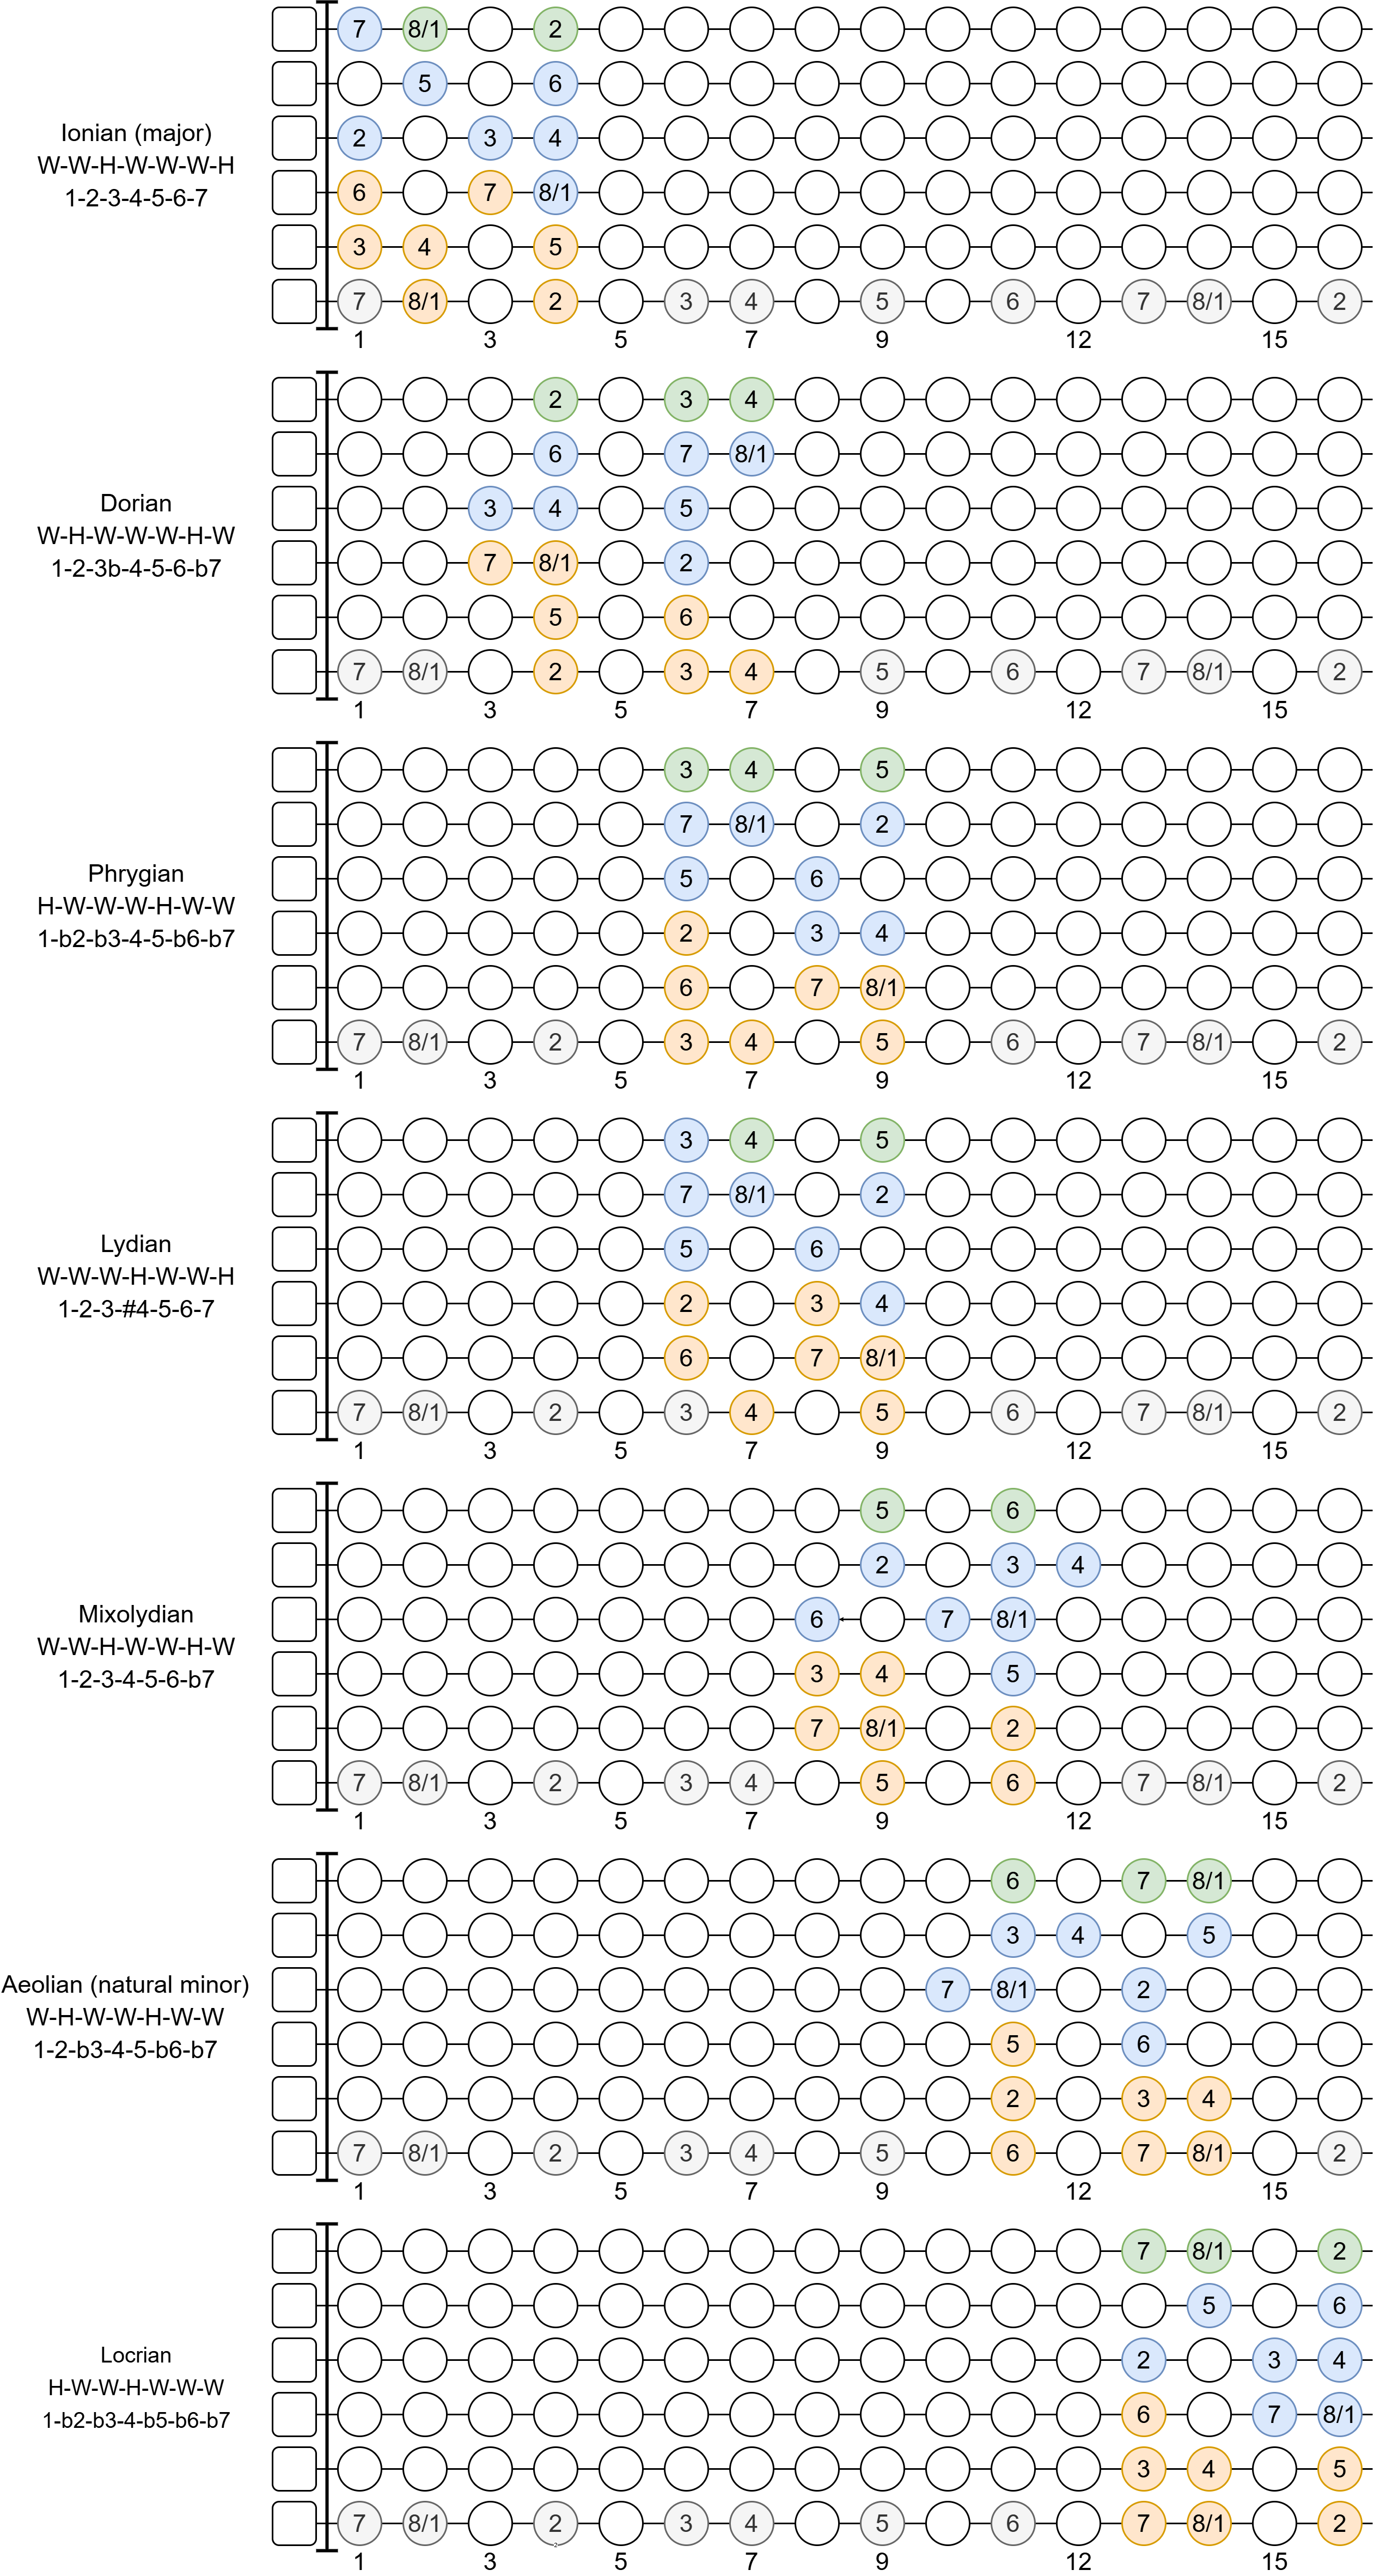
\includegraphics[width=0.9\textwidth]{../../Images/guitar_mode_all.png}
	\caption{Diatonic modes on the guitar}
	\label{fig:guitar_diatonic_modes_on_guitar}
\end{figure}

\clearpage

Note that modes in general are not considered scales per se. Look at the 1, 3, and 5 notes in each mode. This triad is either a major or minor triad (except the locrian mode which is a diminished triad).

\section{CAGED}
TODO